\documentclass[preprint,12pt]{elsarticle}
% The rebuilt manuscript (Brief 29, 20 November 2026). Every number in the text, the tables and the appendix is traced
% to a results, inputs or predictions file by manuscript/numbers_check.py --rebuild; the figures are drawn by
% src/make_rebuild_figures.py and the tables by src/make_rebuild_tables.py from the results files.
\usepackage[T1]{fontenc}
\usepackage{lmodern}
\usepackage{amsmath}
\usepackage{graphicx}
\usepackage{booktabs}
\usepackage{longtable}
\usepackage{textcomp}
\usepackage{xurl}
\usepackage[hidelinks]{hyperref}
\newcommand{\degC}{\,\textdegree C}
\biboptions{sort&compress}
\setlength{\emergencystretch}{1.5em}
\makeatletter
\def\ps@pprintTitle{\let\@oddhead\@empty\let\@evenhead\@empty\def\@oddfoot{\reset@font\hfil\thepage\hfil}\let\@evenfoot\@oddfoot}
\makeatother

\begin{document}

\begin{frontmatter}

\title{The heat a neighbouring lithium-ion cell needs for thermal runaway propagation depends on how the cell is modelled}

\author{Siddharth Satte}
\ead{siddharth161204@gmail.com}
\address{Independent researcher, Pune, Maharashtra, India}

\begin{abstract}
%ABSTRACT-START
Propagation models treat a failing lithium-ion cell's neighbour as one temperature (lumped) or a resolved field. For two touching LG M50 cells with published kinetics, against sixteen two-cell tests, this paper asks how much heat each needs. With the failing cell's energy held to calorimetry, conduction and radiation leave the neighbour at least 29~K short; the rest must come from the ejecta or other paths. About 7~kJ over 21.4~s makes the resolved neighbour run away, 1.5 and 1.7 times the lumped one's need in two tests. Conduction into the surface layer sets the resolved neighbour's hot-spot threshold, within 3\,\% of a conduction model. The lumped neighbour runs away once heated to 218.5\degC, where reaction heat outruns losses. The kinetics' uncertainty moves that temperature by 6.1~K; matching the models needs every rate evaluated over 17.5~K hotter. At the measured times the resolved neighbour needs 4.1 to 8.1~kJ, the lumped one 0.2 to 6.0~kJ. Published inputs let every such path deliver 27.9~kJ or more, so neither tests nor inputs decide. The one published history jumps from 37~K below the resolved neighbour's far side. A facing-side heat flux measurement would decide.
%ABSTRACT-END
\end{abstract}

\begin{keyword}
Thermal runaway propagation \sep Lithium-ion battery \sep Battery safety \sep Cell-to-cell heat transfer \sep Decomposition kinetics \sep Reduced-order model \sep Vent ejecta
\end{keyword}

\end{frontmatter}

%BODY-START
\section{Introduction}
\label{sec:intro}

When one cell in a lithium-ion pack runs away, the pack's safety turns on whether its neighbours follow, and models of the pack are used to judge whether and when they do~\cite{feng2015propagation,coman2017modelling,mishra2021multimode,hoelle2023simulation}. The question such a model has to answer is how much heat must reach a neighbour for the neighbour to follow, and whether a model built only from published inputs can say. This paper puts that question to a pair of cylindrical cells for which sixteen propagation tests have been published.

Pack models represent each cell as one temperature or resolve it, and let a neighbour run away when its temperature reaches an onset value or when Arrhenius heat sources outrun its losses. Their heat paths are conduction through contacts, tabs and holders, radiation and convection~\cite{mishra2021multimode}. Some represent what the failing cell vents, as a share of its energy carried off with the ejecta~\cite{coman2017modelling} or as the vent gas and its reactions~\cite{kim2021venting}, and some the gas layer that vaporising electrolyte forms between the roll and the can~\cite{hoelle2023simulation}. Calorimetry shows why the vent matters: fractional thermal runaway calorimetry of 18650 cells finds that typically 20 to 30\,\% of the total energy leaves through the casing and the rest with the ejecta~\cite{walker2019decoupling}, the Battery Failure Databank holds such measurements for many cells, the LG M50 among them~\cite{finegan2024databank}, and burning vent gas can add to them in open air~\cite{vendra2022numerical,chen2020experimental}. Propagation tests of modules report the order and timing of failures and how barriers, sleeves and sidewall breaches change them~\cite{lamb2015failure,said2019cascading,torrescastro2020passive,read2024barrier,schoberl2024propagation,allen2025sleeves}. None of these sources, as far as they could be read, measures what part of the ejected energy reaches a neighbour, so a model has to choose it.

Fransson et al.~\cite{fransson2024exploring} ran sixteen two-cell propagation tests of LG M50 cells in direct contact, joined by welded tabs, eight in series and eight in parallel, in a rig built for high-speed X-ray imaging~\cite{pfaff2023insitu}. For each test they report whether the neighbour propagated, when, and the two cells' maximum surface temperatures from one thermocouple per cell. Nine propagated, 147 to 342~s after the trigger's runaway. Read, Jones and Marco~\cite{read2024sidewall} report tests of a seven-cell module of the same cell in which propagation followed the trigger's sidewall rupture. Such datasets allow a model to be set against tests one by one.

Whether a neighbour follows also depends on how a model represents it. A lumped neighbour holds the cell's whole inventory at one temperature; a resolved neighbour has a hot region where the heat arrives and a cooler bulk, and its runaway can be read at its hottest point or for the cell as a whole. The decomposition reactions that turn heating into runaway form a network of the SEI, the electrolyte, the electrodes and the separator~\cite{feng2018mechanism}. Koenig, Zhao and Deng~\cite{koenig2025uncertainty} inferred such a network from calorimetry with a Bayesian chemical reaction neural network and published its posterior, which lets the kinetic uncertainty be carried into a cell model.

This paper models the M50 pair with those kinetics and reads the neighbour's runaway three ways: at the hottest point of a resolved neighbour, for a lumped neighbour, and for the resolved neighbour as a whole. It asks, in turn, whether conduction and radiation from the failing cell's body are enough; how much heat must be delivered to the neighbour's facing side for each reading, why the three differ and by how much; what the sixteen tests then say; what physical paths could deliver that heat; and whether a reduced model can stand for the resolved neighbour. It reports what each reading needs and which measurement would decide between them.

\section{Methods}
\label{sec:methods}

\subsection{Tests, cells and trigger}
\label{sec:tests}

The tests are those of Fransson et al.~\cite{fransson2024exploring} (Table~\ref{tab:tests}): two LG M50 cells (21700 format) side by side with their cans touching along a line, joined by welded tabs, the trigger penetrated by a nail, a thermocouple at the middle of each cell's surface at an angle the paper does not give, and times counted from the trigger's runaway. The neighbours of five of the seven tests that did not propagate peaked at 71 to 133\degC; the other two report 626 and 808\degC, which may not be the neighbour's surface, and are treated as exploratory. One history of a neighbour before propagation is published, PT-Exp4's, in the paper's supplementary Figure~10; it was read out of the figure's vector paths twice, by separate code, to 2.47~K and 0.45~s. Tests are named as Fransson et al.\ name them, without the prefix M50.

The failing cell, the trigger, is one temperature that releases its body energy $E_\mathrm{b}$ inside itself as a triangular pulse over 21.39~s, the mean rise time of the two trigger records that the supplement draws. Each test has its own trigger: the $E_\mathrm{b}$ that puts the model's trigger at the test's measured trigger peak at the central contact (below), 9.0 to 54.3~kJ (Table~\ref{tab:tests}). In thirteen of the sixteen tests it exceeds 33.2~kJ, the largest body energy the Battery Failure Databank measured in the ten nail tests of this cell~\cite{finegan2024databank}, probably because the trigger's flame heats the thermocouple the energy is matched to; the same tests are therefore also run with the body energy held to 33.2~kJ. The Databank's median energy carried by this cell's ejecta is 76.74~kJ and its largest 89.34~kJ. The trigger's temperature history is computed once, from the trigger and a lumped neighbour without reaction, and imposed on every neighbour model: what the neighbour does is not fed back to the trigger.

\subsection{Three readings of the neighbour}
\label{sec:neighbour}

The neighbour is solved twice from the same trigger history (Fig.~\ref{fig:geometry}a), with the parameters of Table~\ref{tab:params}. The lumped neighbour is one temperature $T$:
\begin{equation}
\begin{split}
C\frac{\mathrm{d}T}{\mathrm{d}t}={}&(G_c+G_t)(T_1-T)+\varepsilon^2\sigma F A_\ell\,(T_1^4-T^4)\\
&-h_a A_a(T-T_a)-\varepsilon\sigma A_r(T^4-T_a^4)+m\,\dot q_r+P(t),
\end{split}
\label{eq:lumped}
\end{equation}
where $T_1$ is the trigger's temperature, $C=61.75$~J\,K$^{-1}$ the cell's heat capacity and $m$ its mass, $G_c$ the conductance of the contact and its air wedge integrated over the can, $G_t$ that of the welded tabs, $F$ the view factor between the cans and $A_\ell$ the lateral area, $h_a$, $A_a$ and $A_r$ the room's convection coefficient and the areas that convect and radiate to the room at $T_a=25$\degC, $\dot q_r$ the reaction heat per unit mass (Section~\ref{sec:kinetics}) and $P(t)$ the delivered heat (Section~\ref{sec:delivery}). The resolved neighbour is a three-dimensional half model, symmetric about the plane through both axes, of linear tetrahedral finite elements on 19,355 nodes: an anisotropic roll inside a 0.25~mm steel can,
\begin{equation}
\rho c\,\frac{\partial T}{\partial t}=\nabla\cdot(\mathbf{k}\,\nabla T)+\rho\,\dot q_r ,
\label{eq:resolved}
\end{equation}
with the conductivity $\mathbf{k}$ 1.3~W\,m$^{-1}$\,K$^{-1}$ across the layers and 25~W\,m$^{-1}$\,K$^{-1}$ along them and the same total heat capacity. On the can, within 45\textdegree{} of the line of contact the heat flux to the trigger is $h(\theta)(T-T_1)$ with
\begin{equation}
h(\theta)=\frac{k_\mathrm{air}}{\delta(\theta)+k_\mathrm{air}/h_c},\qquad \delta(\theta)=2R(1-\cos\theta),
\label{eq:contact}
\end{equation}
a steel-on-steel contact conductance $h_c$ in series with the air in the wedge of width $\delta$ at angle $\theta$ from the line of contact; $h_c$ is 200, 2,000 or 3,700~W\,m$^{-2}$\,K$^{-1}$ for the low, central and high contact, the range of a textbook's table~\cite[Table~2.1]{lienhard2024heat}, since no conductance between cylindrical cells in contact was found. Beyond 45\textdegree{} the can loses heat to the room by convection; everywhere it radiates to the room and receives the trigger's radiation shared over $\theta$ by the local view factor. The tabs are conductances to the trigger at weld discs at the centre of the cap and the base, one tab in series and two in parallel. Time is stepped by backward Euler with a lumped capacity, the reaction integrated node by node in sub-steps that keep any node's reaction heating within 1~K a step. \ref{app:model} gives the remaining approximations.

Three criteria read the neighbour's runaway, each at 255.7\degC, the lower edge of the internal-short band of the kinetic source~\cite{koenig2025uncertainty}, within 900~s of the trigger's release (Fig.~\ref{fig:geometry}b). The local criterion is met when the resolved neighbour's hottest point reaches it. The lumped criterion is met when the lumped neighbour does. The resolved criterion is met when the resolved neighbour's mean temperature does, the mean weighted by heat capacity, which is the cell's stored heat over its heat capacity and the quantity the lumped temperature stands for. The far face is the resolved neighbour's surface point at mid-length opposite the line of contact.

\begin{figure}[!tbp]
\centering
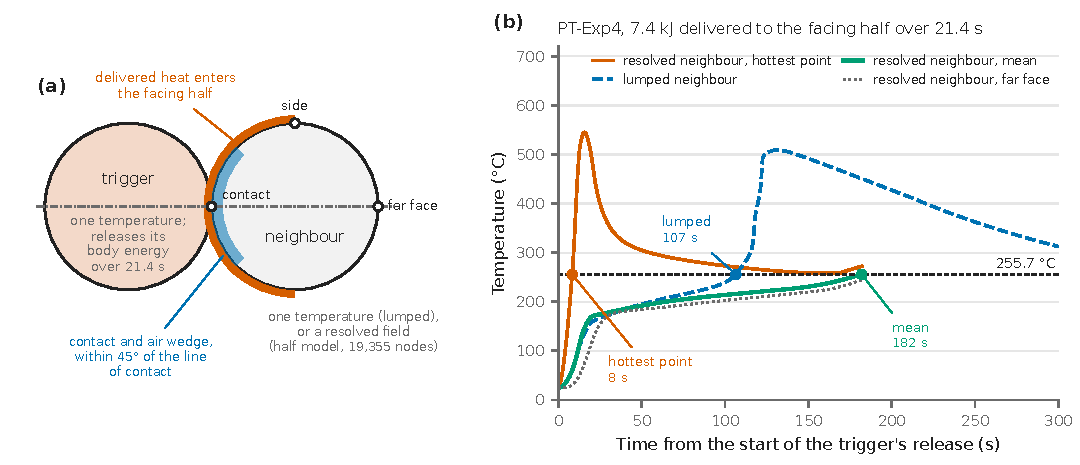
\includegraphics[width=\textwidth]{figures/fig1.pdf}
\caption{The model and its three readings. (a) The pair at mid-length: the trigger is one temperature; the neighbour is solved as one temperature and as a resolved half model, symmetric about the dash-dotted plane; heat is delivered through the half of its can that faces the trigger; within 45\textdegree{} of the line of contact the cans exchange heat through the contact and its air wedge. The three points at mid-length bracket the unreported angle of the measured thermocouple. (b) One run, PT-Exp4 with 7.4~kJ delivered over 21.4~s: the resolved neighbour's hottest point reaches 255.7\degC{} at 8~s, the lumped neighbour at 107~s and the resolved neighbour's mean at 182~s.}
\label{fig:geometry}
\end{figure}

\IfFileExists{tables/t1_tests.tex}{\begin{table}[!tbp]
\centering
\footnotesize
\setlength{\tabcolsep}{2.6pt}
\caption{The sixteen two-cell tests of LG M50 cells of Fransson et al.~\cite{fransson2024exploring} (their Tables 3 and 4), and the body energy $E_\mathrm{b}$ that puts the model's trigger at the measured trigger peak at the central contact when released over 21.39~s. Times run from the trigger's runaway to the neighbour's. The two maxima marked $^{a}$ may not be the neighbour's surface and are treated as exploratory. Category, Fransson et al.'s failure category: 1, the trigger's nail-penetration failure; 2, failure in the propagating cell; 4, sidewall rupture of the trigger; c.m., ``cell movement'' in the X-ray camera's field of view, given in place of a category; a dash, none given.}
\label{tab:tests}
\begin{tabular}{llrrlrrc}
\toprule
Test & Connection & Trigger peak & $E_\mathrm{b}$ & Propagated & Time & Neighbour peak & Category \\
 & & (\textdegree C) & (kJ) & & (s) & (\textdegree C) & \\
\midrule
PT-Exp1 & parallel & 164 & 9.0 & no &  & 71 & c.m. \\
PT-Exp2 & parallel & 679 & 43.4 & no &  & 808$^{a}$ & 1 \\
PT-Exp3 & parallel & 507 & 31.6 & no &  & 118 & 4 \\
PT-Exp4 & parallel & 630 & 40.0 & yes & 272 & 607 & 4 \\
PP-Exp1 & parallel & 787 & 51.1 & yes & 152 & 381 & c.m. \\
PP-Exp2 & parallel & 644 & 41.0 & yes & 147 & 699 & 2 \\
PP-Exp3 & parallel & 686 & 43.9 & no &  & 105 & -- \\
PP-Exp4 & parallel & 728 & 46.9 & yes & 275 & 523 & 2 \\
\midrule
ST-Exp1 & series & 788 & 51.1 & no &  & 128 & 1 \\
ST-Exp2 & series & 723 & 46.5 & no &  & 133 & 4 \\
ST-Exp3 & series & 282 & 16.6 & yes & 177 & 763 & 1 \\
ST-Exp4 & series & 756 & 48.8 & yes & 342 & 733 & 1 \\
SP-Exp1 & series & 728 & 46.8 & yes & 223 & 546 & 2 \\
SP-Exp2 & series & 755 & 48.7 & yes & 149 & 698 & c.m. \\
SP-Exp3 & series & 832 & 54.3 & yes & 210 & 420 & c.m. \\
SP-Exp4 & series & 625 & 39.6 & no &  & 626$^{a}$ & -- \\
\bottomrule
\end{tabular}
\end{table}
}{}

\IfFileExists{tables/t2_parameters.tex}{\begin{table}[!tbp]
\centering
\scriptsize
\caption{The model's parameters and their sources. The two-cell geometry and its solver are those of an earlier, archived study by the author~\cite{satte2026twocell}, whose cells stood apart and were joined by busbars; here the cans touch along a line and welded tabs join the cells, as in the tests. $^{a}$, a value that study set without a primary source, held here as an assumption.}
\label{tab:params}
\renewcommand{\arraystretch}{0.9}
\setlength{\tabcolsep}{4pt}
\begin{tabular}{>{\raggedright\arraybackslash}p{0.28\textwidth}>{\raggedright\arraybackslash}p{0.43\textwidth}>{\raggedright\arraybackslash}p{0.21\textwidth}}
\toprule
Quantity & Value & Source \\
\midrule
\multicolumn{3}{l}{\textit{Geometry and cells}} \\
Cell diameter and length & 21.1 and 70.1 mm & \cite{oregan2022thermal} \\
Can wall & 0.25 mm & \cite[Table 1]{finegan2024databank} \\
Can: conductivity; mass and specific heat & 15 W\,m$^{-1}$\,K$^{-1}$, a stainless steel's (no source gives the grade); 9 g, 500 J\,kg$^{-1}$\,K$^{-1}$ & assumed$^{a}$ \\
Roll conductivity across and along the layers & 1.3 and 25 W\,m$^{-1}$\,K$^{-1}$ & \cite{oregan2022thermal,chen2021simplified} \\
Cell heat capacity & 61.75 J\,K$^{-1}$ (65 g at 950 J\,kg$^{-1}$\,K$^{-1}$; the Databank's cells weighed 68.05 to 68.52 g before their tests~\cite{finegan2024databank}) & \cite{oregan2022thermal}; mass assumed$^{a}$ \\
Resolved neighbour & half model, 19,355 nodes & this study \\
\multicolumn{3}{l}{\textit{Heat paths}} \\
Contact conductance between the cans, $h_c$ & 200, 2,000, 3,700 W\,m$^{-2}$\,K$^{-1}$ (low, central, high) & \cite[Table 2.1]{lienhard2024heat} \\
Air in the wedge beside the contact & 0.03 W\,m$^{-1}$\,K$^{-1}$ & assumed$^{a}$ \\
Contact sector, either side of the line of contact & 45\textdegree & assumed$^{a}$ \\
Welded tabs: series one, parallel two & 6.8 mW\,K$^{-1}$ per tab (5 and 10 as brackets) & assumed$^{a}$ \\
View factor between the cans; emissivity & 0.1817; 0.8 & \cite{bergman2011fundamentals}; assumed$^{a}$, as in \cite{chen2021simplified} \\
Room convection; ambient and start & 10 W\,m$^{-2}$\,K$^{-1}$; 25\textdegree C & assumed$^{a}$ \\
\multicolumn{3}{l}{\textit{Trigger}} \\
Model and release & one temperature; triangular over 21.39 s & \cite{fransson2024exploring} \\
Body energy $E_\mathrm{b}$ & 9.0 to 54.3 kJ, one per test (Table 1); 33.2 kJ held to calorimetry & \cite{fransson2024exploring,finegan2024databank} \\
\multicolumn{3}{l}{\textit{Kinetics}} \\
Model & Bayesian chemical reaction neural network: posterior mean, and 200 joint draws & \cite{koenig2025uncertainty} \\
Reactant masses; initial SEI amount & per 720 g reference cell; 0.15 of the source's normalised amount (fresh), 0 (aged) & \cite{koenig2025uncertainty} \\
Runaway level; window & 255.7\textdegree C; within 900 s & \cite{koenig2025uncertainty}; this study \\
\multicolumn{3}{l}{\textit{Delivered heat}} \\
Region & the half of the neighbour's can facing the trigger, a uniform flux & this study \\
Shapes & triangular over 21.39 s; constant power over 120, 240 or 360 s, the last outlasting the longest combustion reported for a 21700 cell, about 300 s~\cite{chen2023comprehensive}; in PT-Exp4 also the pulse followed by a constant power; for Section~\ref{sec:res-why}, triangular over 5 to 360 s & this study \\
\bottomrule
\end{tabular}
\end{table}
}{}

\subsection{Decomposition kinetics}
\label{sec:kinetics}

The kinetics are the Bayesian chemical reaction neural network of Koenig, Zhao and Deng~\cite{koenig2025uncertainty}, trained on calorimetry of NCM811 and graphite: seven reactions of the anode, electrolyte, SEI and binder, three of the cathode and the separator's melting. Reaction $j$ runs at $r_j=\exp\!\big(\sum_s n_{sj}\ln c_s+\ln A_j+b_j\ln T-E_{a,j}/(RT)\big)$, its species change as $\mathrm{d}c_s/\mathrm{d}t=\sum_j\nu_{sj}r_j$, and its heat enters per unit cell mass as $\dot q_r=\sum_j\Delta H_j r_j m_j/M_\mathrm{ref}$, with $m_j$ the reactant masses of the source's 720~g reference cell. The model is the mean of each parameter over the source's posterior particles; its calorimetry curves reproduce the source's. The posterior enters as 200 joint draws, each one particle of each submodel's file, which treats the three submodels as independent. The SEI starts fresh, at the source's initial amount, or, as a sensitivity, aged, at none.

\subsection{Delivered heat and thresholds}
\label{sec:delivery}

Heat beyond what the trigger's body conducts and radiates, standing for what its ejecta deliver, enters the resolved neighbour as a uniform flux through the half of its can that faces the trigger, and the lumped neighbour receives the same energy $E$. Its shape in time is a triangular pulse over 21.39~s from the start of the trigger's release, a constant power over 120, 240 or 360~s, or, in one test, a pulse followed by a constant power. A threshold is the least delivered energy at which a criterion is met, for a stated shape; a search brackets it between the largest energy run that does not meet the criterion and the smallest that does, and its midpoint is quoted. For a test that propagated, its need is the delivered energy at which a criterion is met at the measured time (within 10~s, or at the threshold where the measured time lies within the search's resolution of it); for a test that did not, the energy at which the far face peaks at the measured maximum (within 5~K). A need is a model quantity: the heat a model must receive to reproduce a test, which the tests do not measure.

\subsection{Reduced models}
\label{sec:reduced}

Four reduced models, built from the same inputs with no parameter fitted, test whether each threshold has a simple mechanism (\ref{app:reduced}). The skin model is the closed form of a semi-infinite solid with the roll's across-layer properties under the delivered flux. The cross-section model is linear conduction in radius and angle at mid-length, with the can, the contact, the wedge, convection and radiation, and neither the reaction nor the axial direction. The ignition temperature $T_\mathrm{ign}$ is the temperature at which the lumped neighbour's reaction heat, with the separator molten, equals its losses. The two-body model runs the trigger and the lumped neighbour without reaction and asks when the neighbour reaches $T_\mathrm{ign}$ with enough heat of the low-temperature cathode reaction left to reach 255.7\degC. The reactive cross-section adds the kinetics, integrated in every cell of the roll, to the cross-section model; it has neither the cell's ends nor its tabs, so it is a cell infinitely long under the conditions at mid-length.

\subsection{Bounds on what each path can deliver}
\label{sec:bounds}

For each path by which the trigger's ejecta or its circuit can heat the facing half, a lower and an upper bound were set on the energy delivered within the pulse's 21.4~s and in total, from published inputs alone, each read at its source and labelled as measured on this cell or on another (Table~\ref{tab:bounds}; the inputs in Supplementary Table~S5). Where no source gives a fraction (a radiant fraction, an absorptivity, the share of vent gas that passes the neighbour, the share of the ejecta that a breach carries), the whole is assumed, so each upper bound is what the published inputs cannot be made to exceed. Radiation was bounded by ray tracing the facing half's view of the region beyond the trigger's end, and convection by Churchill and Bernstein's relation~\cite{churchill1977correlating}.

\subsection{Pre-registration and checks}
\label{sec:prereg}

The study ran in fifteen steps (Supplementary Table~S1). Before each step's runs its predictions, each with the outcome then expected, were committed to a public repository and pushed, and the files were not changed afterwards~\cite{satte2026repo}. Of 98 predictions, 56 held and 42 failed; every one, its expectation and its verdict are in Supplementary Table~S2. The energy account of every run closes to within $2\times10^{-11}$ of the heat taken in. Halving the mesh spacing and every step limit moved the hottest point's peak rise by at most 0.52\,\% and the resolved neighbour's runaway time near its threshold by 1.5\,\%. Registered numbers were recomputed by separate code, and every registered number and verdict was read again by a check that had not drafted the texts.

\section{Results}
\label{sec:results}

\subsection{Conduction and radiation from the trigger's body are not enough}
\label{sec:res-conduction}

With body energies up to 33.2~kJ and the cans in contact, conduction and radiation take neither neighbour to 255.7\degC{} within 900~s in any of 5,248 runs across the contact, tab, release and connection brackets and the 200 kinetic draws: the hottest point peaks at most at 226.7\degC{} and the lumped neighbour at 180.6\degC. With each test's own fitted trigger, conduction carries the hottest point over 255.7\degC{} in the eight tests with the largest fitted triggers (46.5 to 54.3~kJ), within 21.7~s, and the lumped neighbour in two. Held to 33.2~kJ, those eight tests ignite neither neighbour: the hottest point peaks at 191.9 to 192.2\degC{} at the central contact and at 226.4 to 226.7\degC{} at the high contact, 63.5 to 63.8~K and 29.0 to 29.3~K short of 255.7\degC, and the lumped neighbour at 159.8 to 161.8 and 175.9 to 177.4\degC. Even with the fitted triggers and no delivery, the resolved neighbour as a whole runs away in no test at any contact (at the high contact, by the reactive cross-section of Section~\ref{sec:reduced} in ten of the sixteen tests), while nine tests propagated in the rig. Heat beyond what the trigger's body conducts and radiates must therefore reach the neighbour.

\subsection{What a neighbour needs}
\label{sec:res-needs}

With the 21.4~s pulse the three criteria need different energies in every test (Fig.~\ref{fig:thresholds}). The local threshold is zero in the eight tests whose fitted trigger alone carries the hottest point over 255.7\degC, and at most 4.53~kJ (PT-Exp1). The lumped threshold is zero in two tests and at most 12.89~kJ (PT-Exp1). By the reactive cross-section, the resolved neighbour needs 3.5 to 10.8~kJ in all sixteen: more than the lumped threshold in the fourteen tests whose trigger is strong (body energy 31.6 to 54.3~kJ), including 4.5 and 3.5~kJ in the two where the lumped neighbour needs none, and less in the two with weak triggers.

The three-dimensional model confirms this in the four tests it searched. The resolved neighbour runs away above 7.06~kJ in PT-Exp4 (bracket 6.71 to 7.42~kJ) and 6.85~kJ in PP-Exp2 (6.51 to 7.20~kJ), 1.49 and 1.72 times the lumped thresholds of 4.75 and 3.97~kJ, and above 3.88~kJ in SP-Exp3 (3.70 to 4.06~kJ), whose lumped neighbour runs away with no delivery. With PT-Exp4's, PP-Exp2's and SP-Exp3's strong triggers the lumped neighbour runs away in every run of these searches, at 106 to 128~s, releasing 22.4 to 22.6~kJ of reaction heat, where the resolved neighbour has released 4.1 to 4.8~kJ by its own runaway. Only ST-Exp3's weak trigger (16.6~kJ) reverses the order: the resolved neighbour needs 10.28~kJ (9.77 to 10.80~kJ), 0.85 times the lumped neighbour's 12.03~kJ, and at 10.80~kJ it runs away at 61.5~s while the lumped neighbour does not run away.

\begin{figure}[!tbp]
\centering
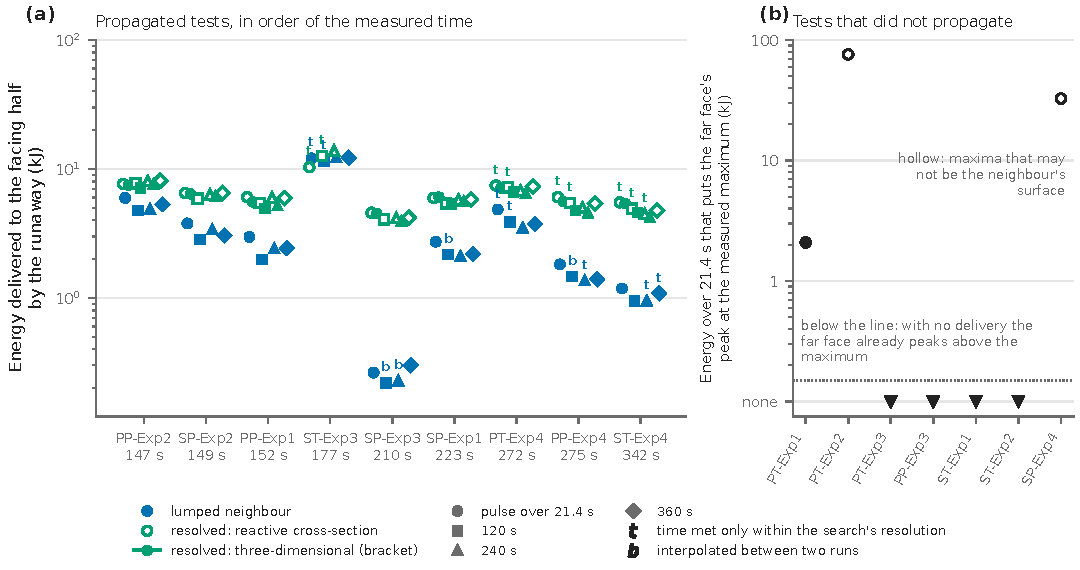
\includegraphics[width=\textwidth]{figures/fig2.pdf}
\caption{The thresholds of the sixteen tests with the 21.4~s pulse, in order of the trigger's fitted body energy (top axis): the least energy delivered to the facing half at which the resolved neighbour's hottest point (triangles), the lumped neighbour (squares) and the resolved neighbour's mean (circles, reactive cross-section; diamonds, three-dimensional model) reach 255.7\degC. Bars are the searches' brackets; a marker at zero means the criterion is met with no delivery. Filled dots below the names mark the tests that propagated.}
\label{fig:thresholds}
\end{figure}

\subsection{Why the three thresholds differ}
\label{sec:res-why}

The local threshold is conduction into a skin (Fig.~\ref{fig:why}a). For PT-Exp1 with deliveries of 5 to 120~s, and for ST-Exp3 and PT-Exp3 at 10 and 60~s, the resolved threshold lies within 3\,\% of the cross-section conduction model, whose value is one end of every final bracket; the delivery's Fourier number $\alpha\tau/a^2$ there runs from 0.025 to 0.60, with $\alpha=5.565\times10^{-7}$~m$^2$\,s$^{-1}$ the roll's diffusivity across its layers, $\tau$ the delivery's duration and $a=10.55$~mm the cell's radius. With the reaction switched off at the upper end of each such search, the hottest point still reaches 255.7\degC{} or falls short by at most 1.1~K, so the reaction plays no part in it. Over 360~s (Fourier number 1.80) the cell heats through: the threshold falls below the conduction model, the hottest point without the reaction peaks 18.9~K short, and with it the crossing comes at 316.5~s on the cell's axis with the mean at 240.1\degC, a runaway inside the cell. The ratio of PT-Exp1's lumped to local threshold accordingly falls from 2.90 at a Fourier number of 0.11 to 1.16 at 0.60 and 0.94 at 1.80.

The lumped threshold is an energy balance to an ignition temperature (Fig.~\ref{fig:why}b,c). The lumped neighbour's reaction heat, with the separator molten, equals its losses at $T_\mathrm{ign}=218.5$\degC{} with the trigger at the neighbour's own temperature (230.4\degC{} with the trigger at 25\degC), and over the 200 kinetic draws $T_\mathrm{ign}$ runs from 215.3 to 221.4\degC{} (central 95\,\%), a span of 6.1~K. At that point the low-temperature cathode reaction gives 73.3\,\% of the reaction heat under the posterior mean. The two-body model, which asks only whether the neighbour reaches $T_\mathrm{ign}$ with enough of that reaction's 2,667~J left to reach 255.7\degC, lies within the larger of 10\,\% and 300~J of the lumped threshold in all 32 searches at the low and high contacts. Because the threshold is the heat that brings the neighbour to $T_\mathrm{ign}$ less what the trigger conducts, it falls by 393 to 456~J per kJ of the trigger's body energy (PT-Exp3, ST-Exp2, PP-Exp3).

The resolved threshold is higher because a resolved cell takes in less through the same contact and does not react as one body. By 250~s the lumped neighbour has taken in 2.1 to 2.3~kJ more than the resolved one through the same conductance, since the resolved cell's contact patch heats toward the trigger's temperature while its mean lags; and the resolved neighbour's reaction heat stays local. The gap is larger than the kinetic uncertainty (Fig.~\ref{fig:why}d). At 5.04~kJ over 21.4~s in PT-Exp4, where the lumped neighbour runs away at 215.6~s, the resolved neighbour runs away under none of four kinetic draws chosen by the rank of their onset (its mean peaks at 191.2 to 192.4\degC) nor with an aged SEI (188.3\degC). Every rate law must be shifted by more than 17.5~K for it to run away there: at 17.5~K its mean peaks at 221.1\degC, and at 20~K it runs away at 270.3~s. That shift is about three times the 6.1~K span of the posterior's ignition temperatures.

\begin{figure}[!tbp]
\centering
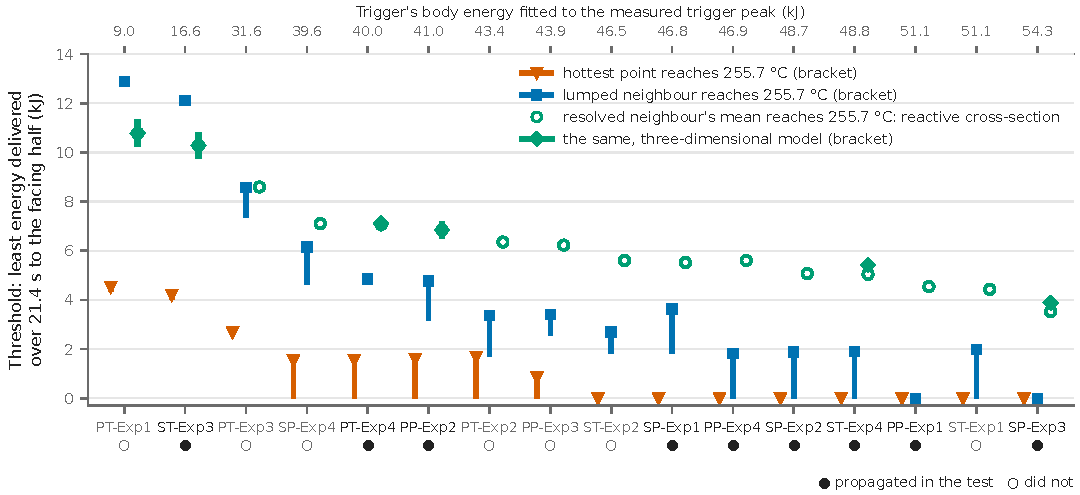
\includegraphics[width=\textwidth]{figures/fig3.pdf}
\caption{Why the thresholds differ. (a) PT-Exp1's local threshold against the delivery's Fourier number: the resolved model with the reaction (brackets) against conduction in the mid-length cross-section and into a semi-infinite skin. (b) The lumped threshold of three tests with the trigger's fitted body energy (hollow) and shifted by 2~kJ either way (filled), with the fall per kJ. (c) The lumped neighbour's ignition temperature over the 200 kinetic draws. (d) That spread beside the shift of every rate law that the resolved neighbour of PT-Exp4 needs to run away at 5.04~kJ: crosses, no runaway; circle, runaway.}
\label{fig:why}
\end{figure}

\subsection{What the sixteen tests then say}
\label{sec:res-tests}

Read through the lumped neighbour, the needs of the sixteen tests vary widely and overlap between the tests that propagated and those that did not. With the 21.4~s pulse the lumped neighbour runs away at the measured time with 0.26 to 5.96~kJ in seven propagated tests, and at its threshold in two (PT-Exp4, 4.66 to 4.85~kJ; ST-Exp3, 11.95 to 12.11~kJ). Of the five tests that did not propagate and report low maxima, four need none, since with no delivery the far face already peaks 13.8 to 56.3~K above their maxima, and PT-Exp1 needs 2.09~kJ, 7.9 times what SP-Exp3 needed to propagate. Over the four delivery shapes these needs span 22- to 64-fold, the largest non-zero over the smallest. Fitted on one connection and scored on the other, no quantity the model yields predicts the outcomes better than one probability for every test by the registered margin of 0.1 in the mean log score: the largest gain is 0.062, with permutation $p$-values of 0.23 to 0.75, and the thresholds mostly restate the trigger's energy (Spearman's $\rho=-0.92$ for the local and $-0.97$ for the lumped).

Read through the resolved neighbour, the needs fall in a narrower band (Fig.~\ref{fig:tests}). For the resolved neighbour to run away at a test's measured time, the reactive cross-section needs 4.1 to 8.1~kJ delivered by then in all twenty-five reproduced cases outside ST-Exp3, whatever the delivery's shape, where the lumped neighbour needs 0.2 to 6.0~kJ in the same cases. With the pulse the resolved need exceeds the lumped one in every test it reproduces, most in SP-Exp3, 4.58 against 0.26~kJ. In ST-Exp3 the resolved neighbour runs away at 114.0~s already at its threshold, before the measured 177~s, so no delivered energy reproduces that test's time.

The one published history sits between the two (Fig.~\ref{fig:history}). PT-Exp4's thermocouple reaches 141.0\degC{} by 45~s and 197.3\degC{} at 271.5~s, when the neighbour's jump begins. With 4.66 and 5.04~kJ over 21.4~s, either side of the lumped neighbour's threshold, the model's far face lies 16.3 and 16.8~K from the record, the root mean square over 0 to 271.5~s, but the resolved neighbour does not run away: with 5.04~kJ its mean peaks at 190.6\degC{} and cools. At 7.42~kJ, the upper end of its own bracket, the resolved neighbour runs away at 181.9~s, before the measured onset at 271.5~s, and its far face's jump begins at 234.1\degC, 36.8~K above the 197.3\degC{} from which the measured neighbour jumped; over 0 to 181.9~s its far face lies 51.4~K from the record. A 5.04~kJ pulse followed by a constant 12.5~W brings the resolved runaway to 255.9~s, and one followed by 10~W to 369.3~s, the two holds having added 2.9 and 3.5~kJ; with 12.5~W the far face's jump begins at 233.6\degC, and it lies 33.1~K from the record over 0 to 255.9~s. The thermocouple's angle is not reported; a post hoc reading of the same run finds the far face the coolest of the model's five probes at mid-length when its jump begins (the two side probes read 235.5 and 235.8\degC), so 36.8~K is the least difference those probes give.

\begin{figure}[!tbp]
\centering
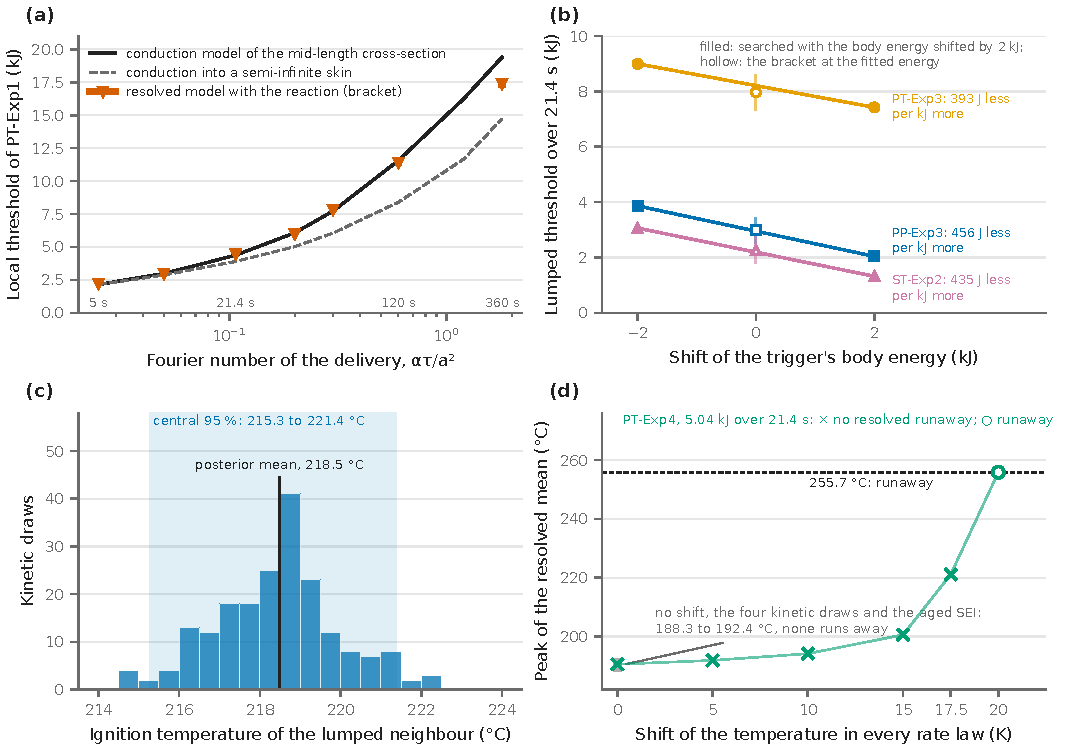
\includegraphics[width=\textwidth]{figures/fig4.pdf}
\caption{What the tests need. (a) For the nine tests that propagated, in order of the measured time: the energy delivered to the facing half by that time at which the lumped neighbour (filled) or the resolved neighbour's mean (hollow, reactive cross-section) reaches 255.7\degC{} at the measured time, for the four delivery shapes; in ST-Exp3 the resolved neighbour runs away before the measured time even at its threshold, which is shown. (b) For the seven tests that did not propagate: the energy delivered over 21.4~s that puts the far face's peak at the measured maximum; hollow, the two maxima that may not be the neighbour's surface; at the bottom, tests whose far face exceeds the maximum with no delivery.}
\label{fig:tests}
\end{figure}

\begin{figure}[!tbp]
\centering
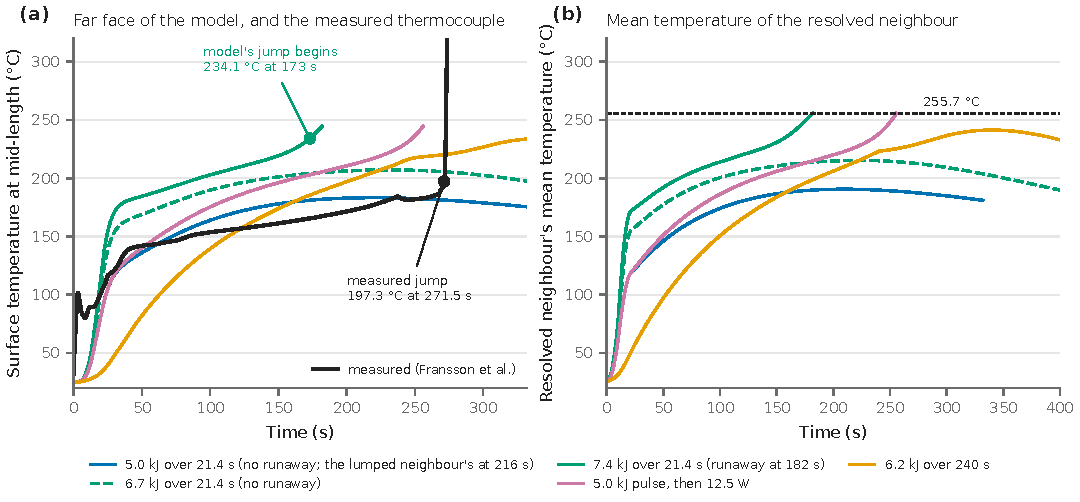
\includegraphics[width=\textwidth]{figures/fig5.pdf}
\caption{PT-Exp4's neighbour. (a) The measured thermocouple (black; Fransson et al.~\cite{fransson2024exploring}, supplementary Figure~10, read from the figure) against the model's far face under five deliveries at the central contact; the circles mark where the model's and the measured jumps begin. (b) The resolved neighbour's mean temperature under the same deliveries; the resolved neighbour runs away where its mean reaches 255.7\degC. The run of 5.0~kJ over 21.4~s was carried to 332~s.}
\label{fig:history}
\end{figure}

\subsection{What could deliver it}
\label{sec:res-paths}

From published inputs alone, what the ejecta can release in this rig is at most 225.8~kJ, and every path but one is bounded only near that (Table~\ref{tab:bounds}, Fig.~\ref{fig:paths}). Within 21.4~s, radiation can deliver at most 27.9~kJ, a black body at 1500\degC{} filling the facing half's view; a flame held on the vent's axis sends at most about 0.37\,\% of its radiation onto the facing half, about 0.85~kJ, but no source places the flame. Gas beside the neighbour can deliver at most 195.5~kJ, a breach's jet facing the neighbour and solids and melt on it 225.8~kJ each, and the neighbour's own discharge in the parallel tests 65.5~kJ. Conduction through the holder is not determinable, because no source gives the material or the contact of the inserts that touch each cell. Within 21.4~s gas, a breach's jet and solids and melt each reach all twelve needs that are not zero; radiation reaches ten and misses only the two exploratory maxima (32.7 and 75.8~kJ); the discharge reaches five of the six parallel needs. Every energy the resolved neighbour needs, under any of the four shapes, is 5.3 to 25.4\,\% of the Databank's median ejected energy and below the least of the bounds within the delivery's duration. The bounds therefore do not choose between the readings of the neighbour.

\IfFileExists{tables/t3_bounds.tex}{\begin{table}[!tbp]
\centering
\footnotesize
\caption{What each path can deliver to the neighbour's facing half, from published inputs alone: the upper bound within the 21.4~s of the pulse and in total (every lower bound is zero), what sets it, and the measurement that would bound it more tightly. What the ejecta can release in the rig is 225.8~kJ, the most calorimetry measured for this cell's ejecta (89.34~kJ)~\cite{finegan2024databank} with the heat of burning the vent gas in open air (at most 136.5~kJ, measured on another 21700 cell)~\cite{vendra2022numerical}; the gas and flame are taken at up to 1500\textdegree C~\cite{chen2020experimental} and the vent gas at up to 398.5~m\,s$^{-1}$~\cite{gillich2024mechanical}.}
\label{tab:bounds}
\renewcommand{\arraystretch}{0.95}
\setlength{\tabcolsep}{4pt}
\begin{tabular}{p{0.19\textwidth}rrp{0.29\textwidth}p{0.19\textwidth}}
\toprule
Path & \multicolumn{1}{c}{21.4 s} & \multicolumn{1}{c}{Total} & What sets the bound & Measurement that would bound it \\
 & (kJ) & (kJ) & & \\
\midrule
Radiation from a vent's jet or flame & 27.9 & 225.8 & a black body at 1500\textdegree C filling the facing half's view, the holder possibly reflecting; held on the vent's axis, about 0.85~kJ & the flame's position and temperature beside the cells \\
Gas beside the neighbour, burning or not & 195.5 & 225.8 & convection at 398.5~m\,s$^{-1}$ with hydrogen's properties~\cite{churchill1977correlating}, at most twice its whole-cylinder mean on one half, and radiation at 1500\textdegree C & the gas's temperature and velocity in the wedges beside the line of contact \\
A breach's jet facing the neighbour & 225.8 & 225.8 & what the ejecta can release; a narrow jet strikes the facing half from a sixth of the circumference & where breaches face and what they carry \\
Solids and melt on or against the facing half & 225.8 & 225.8 & what the ejecta can release; melt falls onto the facing half from half of the circumference & the debris left on the neighbour \\
Conduction through the cell holder & -- & -- & no source gives the inserts' material or contact (247.3~kJ if bounded as the jet and melt are) & the holder's inserts and their contact \\
The neighbour's own discharge (parallel tests) & 65.5 & 65.5 & the rated stored energy (15.6~kJ within 21.4~s if the resistance stayed at its 25\textdegree C value) & the current between parallel cells \\
\bottomrule
\end{tabular}
\end{table}
}{}

\begin{figure}[!tbp]
\centering
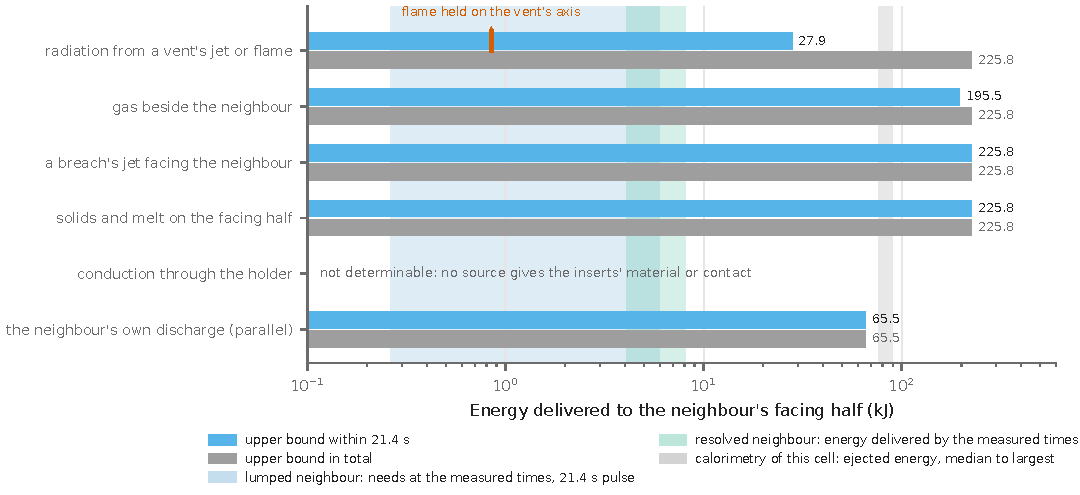
\includegraphics[width=\textwidth]{figures/fig6.pdf}
\caption{What each path can deliver to the neighbour's facing half, from published inputs alone (upper bounds within the pulse's 21.4~s and in total; every lower bound is zero), against what the neighbour models need: the lumped neighbour's needs at the measured times with the pulse, the energy the resolved neighbour needs delivered by the measured times, and the energy calorimetry measured in this cell's ejecta. The mark on the radiation bar is a flame held on the vent's axis.}
\label{fig:paths}
\end{figure}

\subsection{The reactive cross-section as a reduced model}
\label{sec:res-reduced}

The reactive cross-section stands for the resolved neighbour's own runaway (Fig.~\ref{fig:reduced}). Against the 151 central three-dimensional runs that the study had carried past the hottest point's crossing, it gave the same outcome, runaway of the mean within 900~s or none, in all 151. In the 92 runs in which both run away, its runaway comes 1.0~s later on average (5.5~s earlier to 34.5~s later); in the 59 in which neither does, its mean peaks 1.9~K lower on average, and up to 20.7~K lower in the parallel tests, whose tabs it lacks. Its thresholds were registered as the centres of the three-dimensional searches: in three of the four tests the searches' opening two runs, 5\,\% either side of its value, bracketed the threshold, and in SP-Exp3 the threshold lay above both, its value 9.1\,\% below the bracket's midpoint. A run takes 17 to 71~s on one processor core, against 240 to 2,762~s for the three-dimensional runs of the same searches.

\begin{figure}[!tbp]
\centering
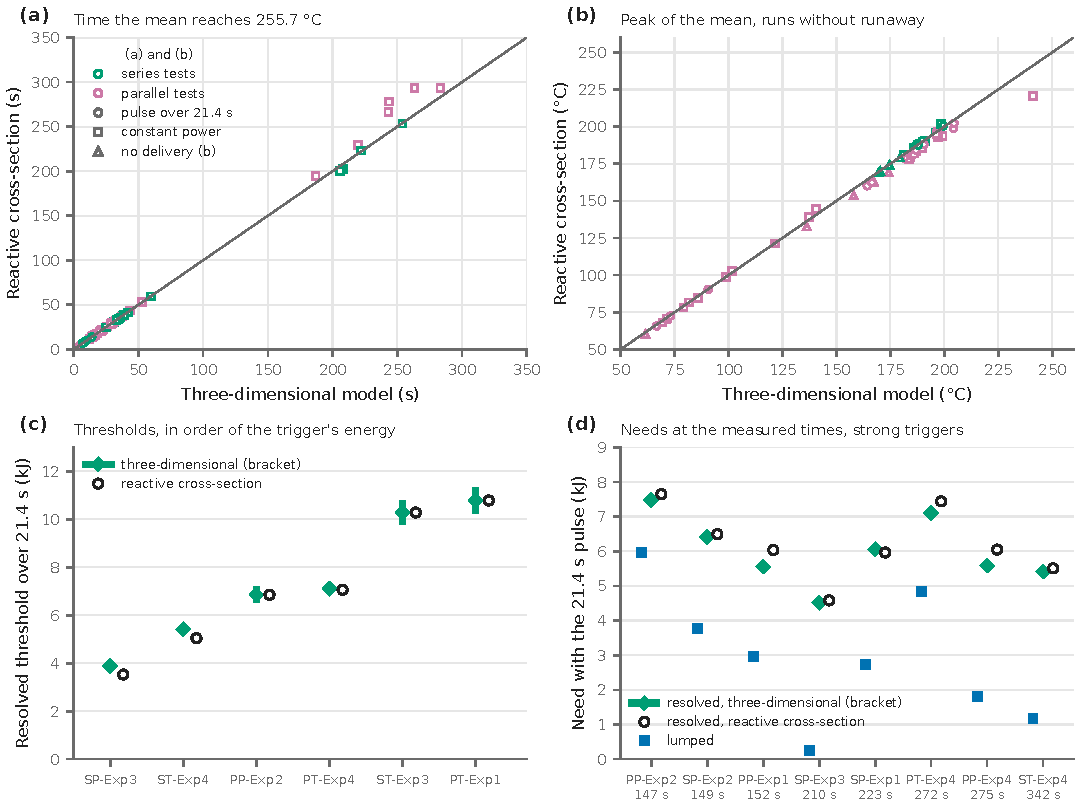
\includegraphics[width=\textwidth]{figures/fig7.pdf}
\caption{The reactive cross-section against the three-dimensional model. (a) The time the resolved neighbour's mean reaches 255.7\degC, in the runs where both models run away. (b) The mean's peak in the runs where neither does. (c) The thresholds of the four tests searched in three dimensions with the 21.4~s pulse. The line in (a) and (b) is equality.}
\label{fig:reduced}
\end{figure}

\section{Discussion}
\label{sec:discussion}

\subsection{The delivered heat as a distribution}
\label{sec:disc-distribution}

A conduction model of these tests lacks the heat their triggers deliver, and the tests do not measure it. Read through a lumped neighbour, what each test needs varies 22- to 64-fold and overlaps between the tests that propagated and those that did not, so a pack model that ignites a neighbour at one delivered share will reproduce some tests and not others. Read through a resolved neighbour, the needs at the measured times fall within 4.1 to 8.1~kJ outside one test, a narrower band, though one the tests cannot yet confirm. Either way the needed energies are a small part of what the ejecta carry: 5.3 to 25.4\,\% of the Databank's median for this cell for the resolved neighbour~\cite{finegan2024databank}. For a different cell and stack, Torres-Castro et al.\ estimated that the next pouch cell absorbed 2.0~kJ on average before it failed~\cite{torrescastro2020passive}, inside the lumped range found here. A pack model would do better to carry the delivered heat as a distribution and to report propagation as a probability; these are implications of the results, and no pack model built on them was run.

\subsection{A neighbour that is not one temperature}
\label{sec:disc-lumped}

The lumped neighbour reaches its runaway with less delivered heat in every test with a strong trigger because it takes in more through the same contact and reacts as one body; its clock's agreement with the measured times belongs to that construction. The resolved neighbour's hottest point crosses within seconds of the delivery, and its mean needs 1.49 to 1.72 times the lumped neighbour's energy. A lumped cell can therefore not serve as the inexpensive model of a cell's own runaway in a module without a correction, while the reactive cross-section, at a small part of the three-dimensional cost, gave the three-dimensional outcome in every archived run it was set against. The measured history fits neither cleanly. Under the lumped neighbour's energy the model's far face lies 16.3 to 16.8~K from PT-Exp4's record but the resolved cell does not run away; at the resolved cell's own runaway its far face is 37~K hotter than the measured surface when the jump begins. A runaway that starts from part of the cell, more heat arriving over a longer time, or rate laws shifted by more than 17.5~K would each reconcile the two; the results here do not choose between them.

\subsection{The measurements that would decide}
\label{sec:disc-measure}

Four measurements would decide between the readings. A heat flux measured on the neighbour's facing side would give the delivered heat directly, in place of a need inferred through a model. The thermocouple's angle would say which part of the neighbour's surface the published maxima and history describe, and so whether the far face's overshoot with no delivery and its 37~K excess at the jump are real. The flame's position and temperature beside the cells would bound radiation by geometry, from 27.9~kJ toward 0.85~kJ. Which way a breach faces, and what it carries, would bound the jet and the melt below what the ejecta can release. Calorimetry of the tests' own triggers would replace a body energy fitted to a thermocouple's peak.

\subsection{Limits}
\label{sec:limits}

One cell type, in one laboratory's rig, carries the comparison, and one published history; that history was read from a figure, and its opening 8.5~s, a spike to 102\degC, are taken as the thermocouple's exposure at the trigger's runaway. The triggers are fitted to one surface thermocouple's peak, beyond the calorimetry's body energy in thirteen of the sixteen tests, and the trigger's history is imposed on the neighbour one way. The contact conductance is a textbook's range, the delivery's region and shapes are choices, and the model has no gas phase, venting or sidewall rupture. The kinetics were trained on NCM811 and graphite, while the M50's negative electrode is silicon and graphite~\cite{oregan2022thermal}, and their draws treat three submodels as independent. Much of what is compared is model against model: the resolved and the lumped neighbour share every input, and only one test's history sets either against a measured temperature.

\section{Conclusions}
\label{sec:conclusions}

\begin{enumerate}
\item With the trigger's body energy held to the largest calorimetry gives for this cell, conduction and radiation leave the neighbour's hottest point at least 29~K short of 255.7\degC.
\item With 21.4~s of delivered heat the resolved neighbour runs away as a whole at 1.49 and 1.72 times the energy the lumped neighbour needs in two tests.
\item Bringing the resolved threshold down to the lumped one would need every rate law shifted by more than 17.5~K, against a 6.1~K span of the posterior's ignition temperatures.
\item At the tests' measured times the resolved neighbour needs 4.1 to 8.1~kJ delivered by then, against 0.2 to 6.0~kJ for the lumped neighbour.
\item Every need lies within the bounds of at least two delivery paths, which published inputs cannot narrow below 27.9~kJ within 21.4~s.
\end{enumerate}

\noindent A heat flux measured on the facing side of a neighbour, with the thermocouple's angle, would decide between the resolved and the lumped reading of these tests.

\appendix
\section{The model's approximations}
\label{app:model}

The trigger is one temperature with the cell's heat capacity; its body energy is released inside it as a triangular pulse, and its temperature history, computed by explicit time steps with a lumped neighbour without reaction, is imposed on every neighbour model. The resolved neighbour's mesh is graded toward the line of contact, the roll is homogeneous and anisotropic, the can is a shell of steel with its own conductance and heat capacity, and the contact sector spans 45\textdegree{} either side of the line of contact, where room convection is removed. Room radiation is lagged one step. Both neighbours hold the same total heat capacity and the same reactant inventory per unit mass. Every run's energy account, the heat taken in through each boundary against the change in stored heat and the reaction heat released, closes to within $2\times10^{-11}$ of the heat taken in.

\section{The reduced models}
\label{app:reduced}

The skin model's peak rise is $\Phi E''/(e\sqrt{\tau})$, with $E''$ the delivered energy per unit area, $\tau$ the pulse's duration, $e=1{,}743$~J\,m$^{-2}$\,K$^{-1}$\,s$^{-1/2}$ the roll's effusivity across its layers and $\Phi=1.2284$ for the triangular pulse; the can enters as a surface layer of 841.7~J\,m$^{-2}$\,K$^{-1}$ with a linear surface loss. It agrees with the cross-section model for the shortest deliveries and falls below it as the delivery lengthens and heat spreads along the layers (Fig.~\ref{fig:why}a). The cross-section model superposes the trigger's conduction on the response to the delivery, with the radiation's nonlinearity taken as the exact secant along the threshold's own solution, so that its threshold is the nonlinear model's at convergence. The ignition temperature solves $m\dot q_r(T_\mathrm{ign})=L(T_\mathrm{ign})$, with $L$ the lumped neighbour's losses to the trigger and the room and the separator molten; the reaction that carries it in every draw is the low-temperature cathode reaction. The reactive cross-section integrates the kinetics in every cell of the roll by the three-dimensional model's own reaction step and feeds their heat back. Every reduced number scored against a three-dimensional run was registered before that run.

\section*{CRediT authorship contribution statement}
Siddharth Satte: Conceptualization, Methodology, Investigation, Resources, Validation, Project administration, Writing~-- review \& editing.

\section*{Declaration of competing interest}
The author declares that he has no known competing financial interests or personal relationships that could have appeared to influence the work reported in this paper.

\section*{Funding}
This research did not receive any specific grant from funding agencies in the public, commercial, or not-for-profit sectors.

\section*{Data availability}
The code, inputs, run records, checks and decisions of every step are archived at Zenodo, \url{https://doi.org/10.5281/zenodo.23279455} (all versions; version 1.11.0, \url{https://doi.org/10.5281/zenodo.24368356}, holds every result used here), and in the repository \url{https://github.com/siddharth161204-wq/m50-neighbour-onset-kinetics}~\cite{satte2026repo}. The two-cell geometry is archived at \url{https://doi.org/10.5281/zenodo.23253738}~\cite{satte2026twocell}.

\section*{Acknowledgements}
The measured tests are those of Fransson et al.~\cite{fransson2024exploring}, published under CC~BY~4.0. The kinetic posterior files are the supplementary data of Koenig, Zhao and Deng~\cite{koenig2025uncertainty}. The Battery Failure Databank is provided by the U.S. Department of Energy's National Renewable Energy Laboratory, operated by Alliance for Sustainable Energy, LLC (DOE/\allowbreak NREL/\allowbreak ALLIANCE)~\cite{finegan2024databank}.

\section*{Declaration of generative AI and AI-assisted technologies in the manuscript preparation process}
% Left for the author to write (his instruction of 11 November 2026).

%BODY-END

\bibliographystyle{elsarticle-num}
\bibliography{references}

\end{document}
